\chapter{Исследовательская часть}

Технические характеристики устройства, на котором было произведено тестирование разработанного ПО: 

\begin{itemize}
	\item операционная система: macOS Big Sur 11.6.4;
	\item оперативная память: 8 Гб;
	\item 2,4 Ггц 2‑ядерный процессор Intel Core i5 \cite{intel}.
\end{itemize}

Во время тестирования ноутбук был включен в сеть питания.

\section{Время выполнения реализаций алгоритмов}

В таблице \ref{tab:time1} приведено время (мс) работы реализаций параллельного алгоритма блочной сортировки для массивов случайных чисел размеров от 10000 до 50000 элементов. 

\begin{table}[h]
	\begin{center}
		\caption{\label{tab:time1}Результаты замеров времени многопоточного алгоритма блочной сортировки}
		\begin{tabular}{|c|r@{}l|r@{}l|r@{}l|r@{}l|r@{}l|}
		\hline
		Количество потоков & 1&0000 &  2&0000  & 3&0000 & 4&0000 & 5&0000 \\
		\hline
		1  & 1.&3204 & 6.&7280 & 18.&5843 & 32.&6369 & 51.&2648 \\
		\hline
		4  & 1.&0098  & 2.&8004 & 5.&5141 &  9.&4126 & 14.&7643  \\
		\hline
		8  & 1.&3321 & 3.&9422 & 7.&2482 &  9.&7218 & 15.&2290 \\
		\hline
		16  & 1.&2935 & 4.&0348 & 8.&3376 & 11.&5191 & 15.&9671 \\
		\hline
		32  & 1.&3028 & 4.&0505 & 8.&3464 & 13.&4814 & 17.&0147 \\
		\hline
		64  & 1.&2980 & 4.&0466 & 8.&4265 & 13.&9359 & 19.&9160 \\
		\hline
		\end{tabular}
	\end{center}
\end{table}

Наилучшее время параллельные алгоритмы показали на 4 потоках, что соответствует количеству логических ядер компьютера, на котором проводилось тестирование. 
Время работы (мс) алгоритма однопоточной реализации и реализации с использованием оптимального количества ядер представлены в таблице \ref{tab:time2}.

\begin{table}[h]
	\begin{center}
		\caption{\label{tab:time2}Результаты замеров времени однопоточной и многопоточной реализаций алгоритма сортировки}
		\begin{tabular}{|c|r@{}l|r@{}l|}
		\hline
		Размер & 1 по&ток &  4 по&тока \\
		\hline
		10000 & 1.&3653 & 1.&0098 \\
		\hline
		20000 & 6.&7280 & 2.&8004 \\
		\hline
		30000 & 18.&5843 & 5.&5141 \\
		\hline
		40000 & 32.&6369 & 9.&4126 \\
		\hline
		50000 & 51.&2648 & 14.&7643 \\
		\hline
		\end{tabular}
	\end{center}
\end{table}

На рисунке \ref{fig:graph1} изображены графики времени работы однопоточного алгоритма сортировки и реализации с 4 потоками. 

\begin{figure}[h!]
	\centering
	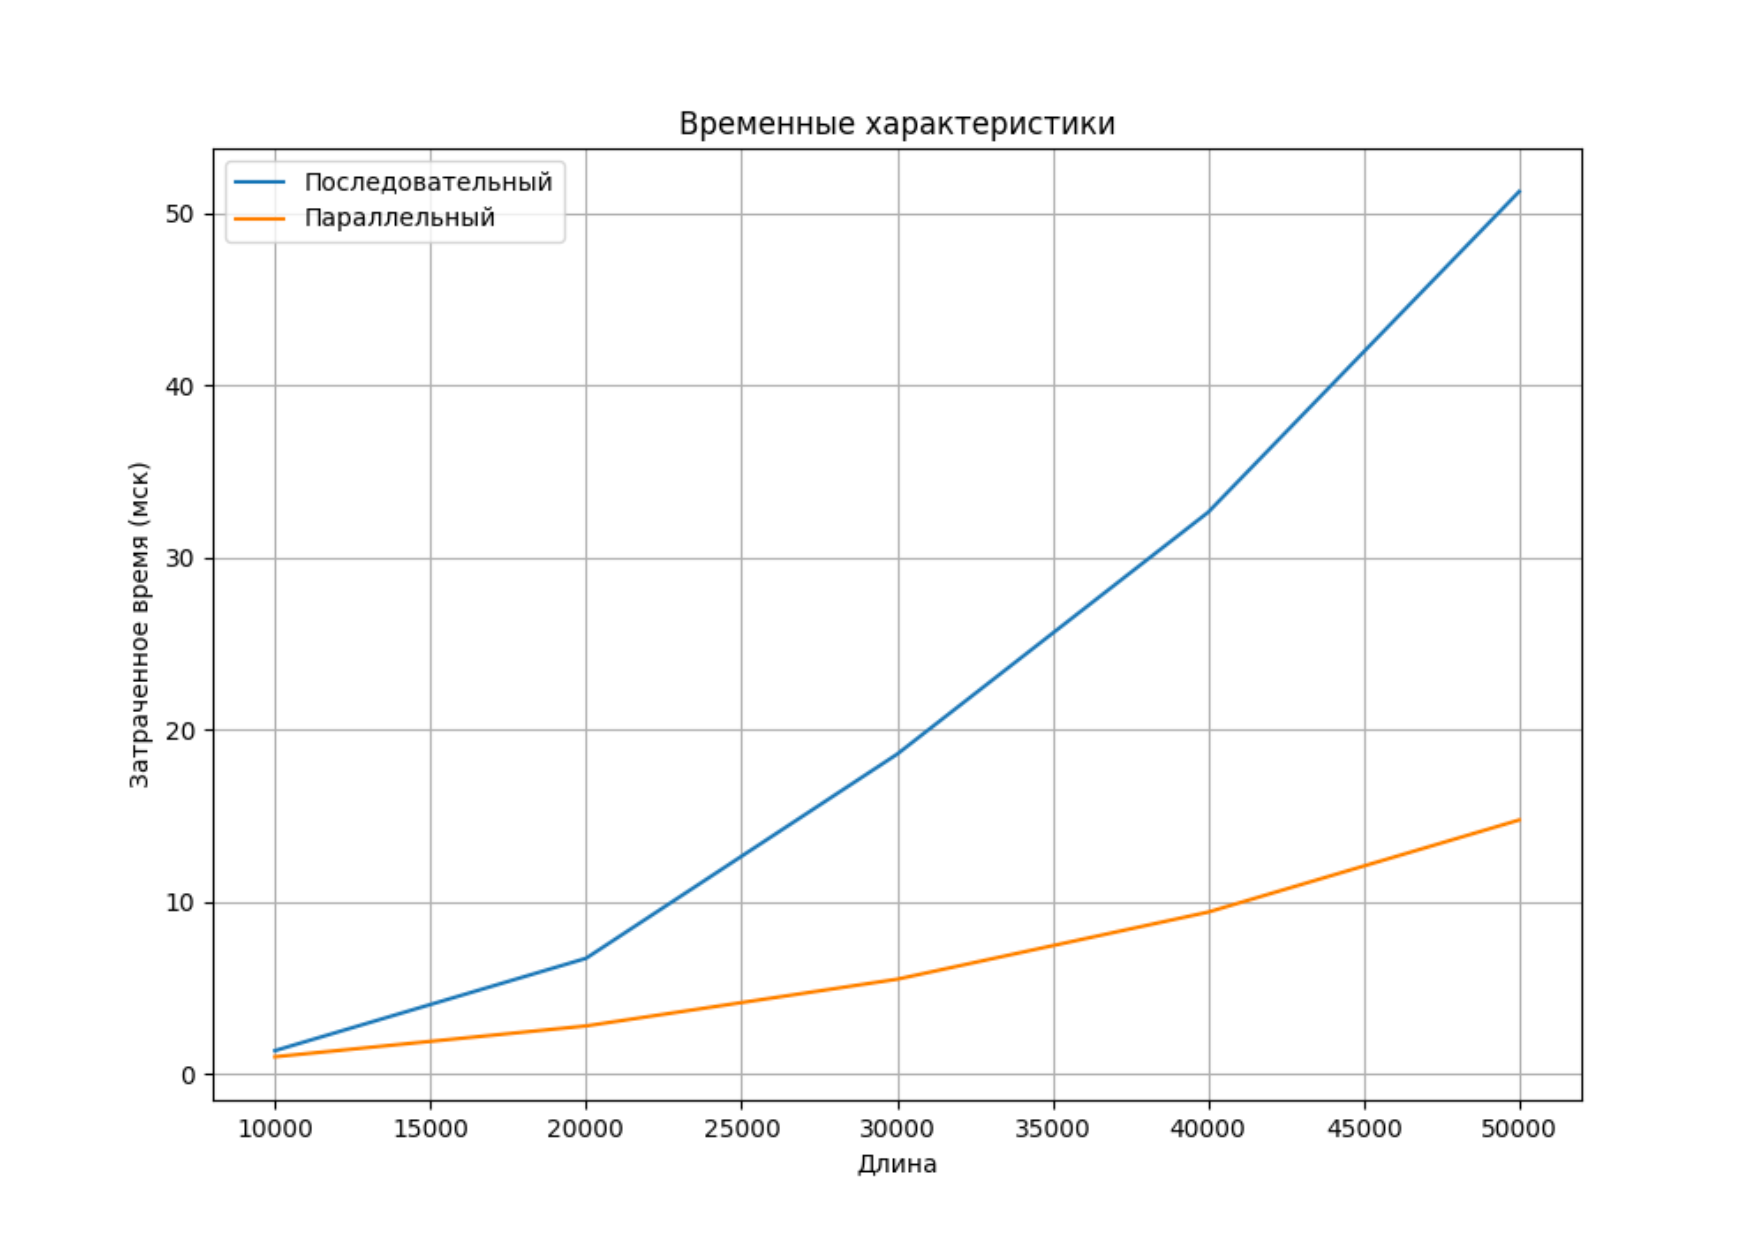
\includegraphics[width=1\linewidth]{img/Plot2.png}
	\caption{Время работы сортировок}
	\label{fig:graph1}
\end{figure}

На рисунке \ref{fig:graph2} изображены графики зависимости времени работы алгоритмов сортировок от количества элементов массивов. 

\begin{figure}[h!]
	\centering
	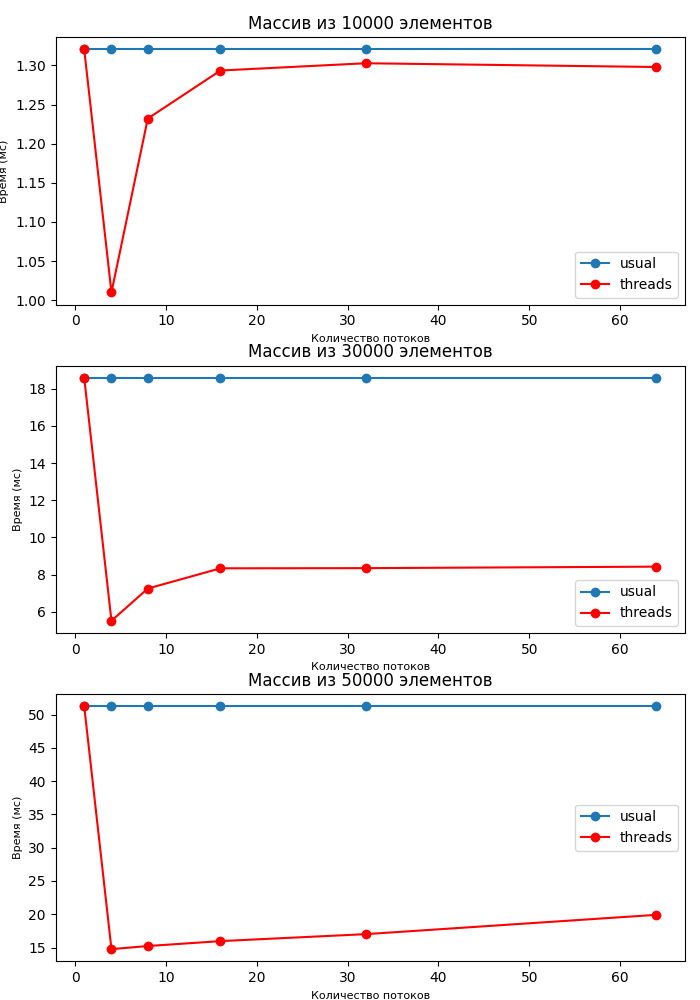
\includegraphics[width=1\linewidth]{img/Plot.png}
	\caption{Время работы сортировок}
	\label{fig:graph2}
\end{figure}

\section*{Вывод}
В данном разделе было произведено сравнение алгоритмов блочной сортировки при однопоточной реализации и многопоточной.

Экспериментально получено, что реализация алгоритма блочной сортировки с использованием параллелизма эффективнее по времени, чем однопоточная. 
Тестирование показало, что распараллеливание алгоритма помогает ускорить работу, а самым выгодным является использование 4 потоков, что совпадает с количеством логических ядер машины, на которой производилось тестирование. 
В среднем многопоточная реализация выигрывает у однопоточной в 3.5 раза. 
